\subsection{Example 1: Port Scan}

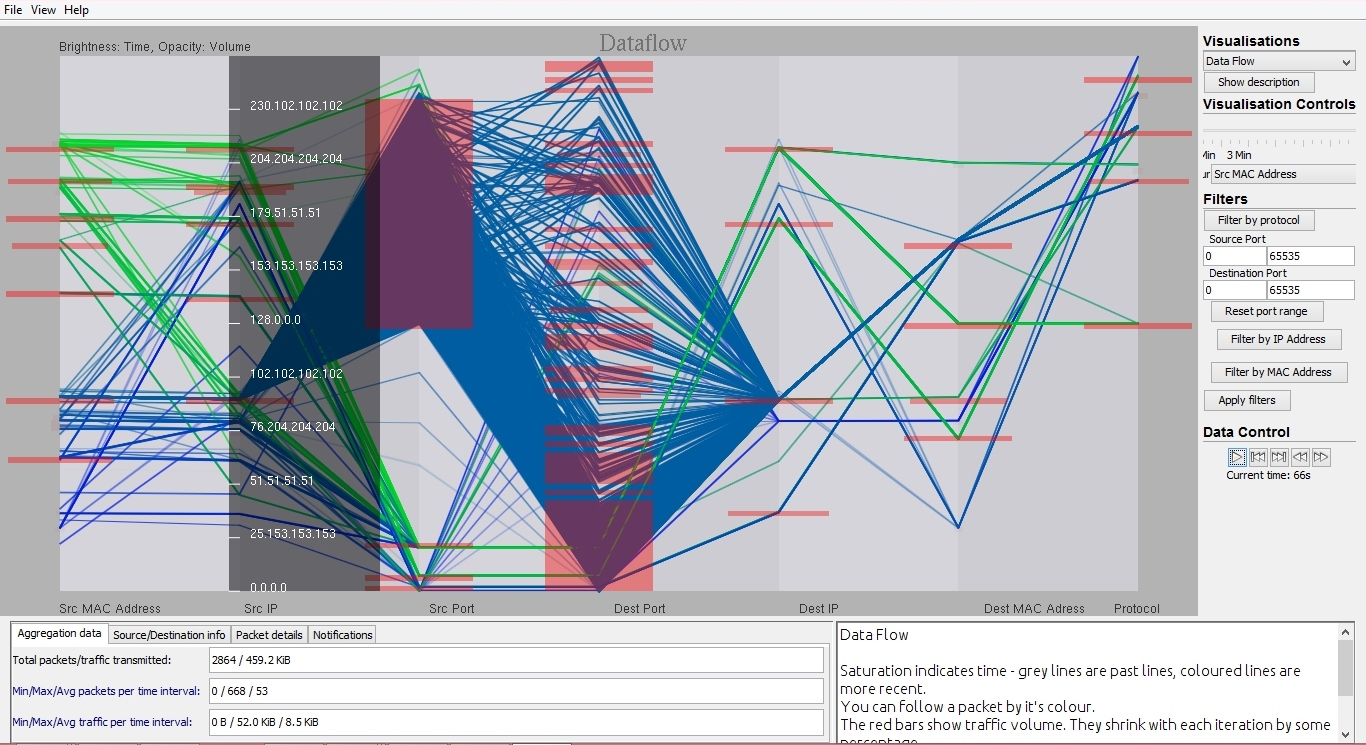
\includegraphics[width=\linewidth]{materials/portscan_detected.jpg}
The analyst can clearly see that a port scan has occured.

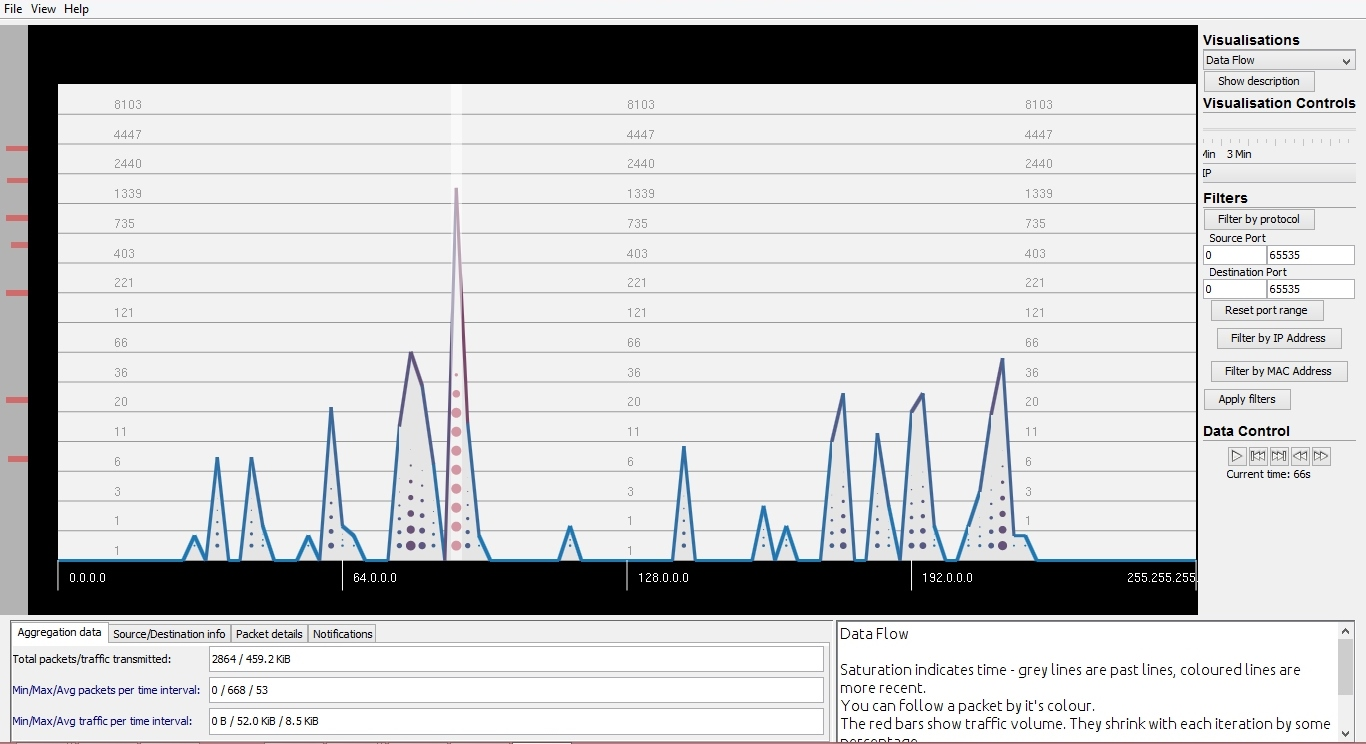
\includegraphics[width=\linewidth]{materials/portscan_identify.jpg}
By visualising the distribution of source IP's he can distinguish a spike in the network traffic for a small IP range.

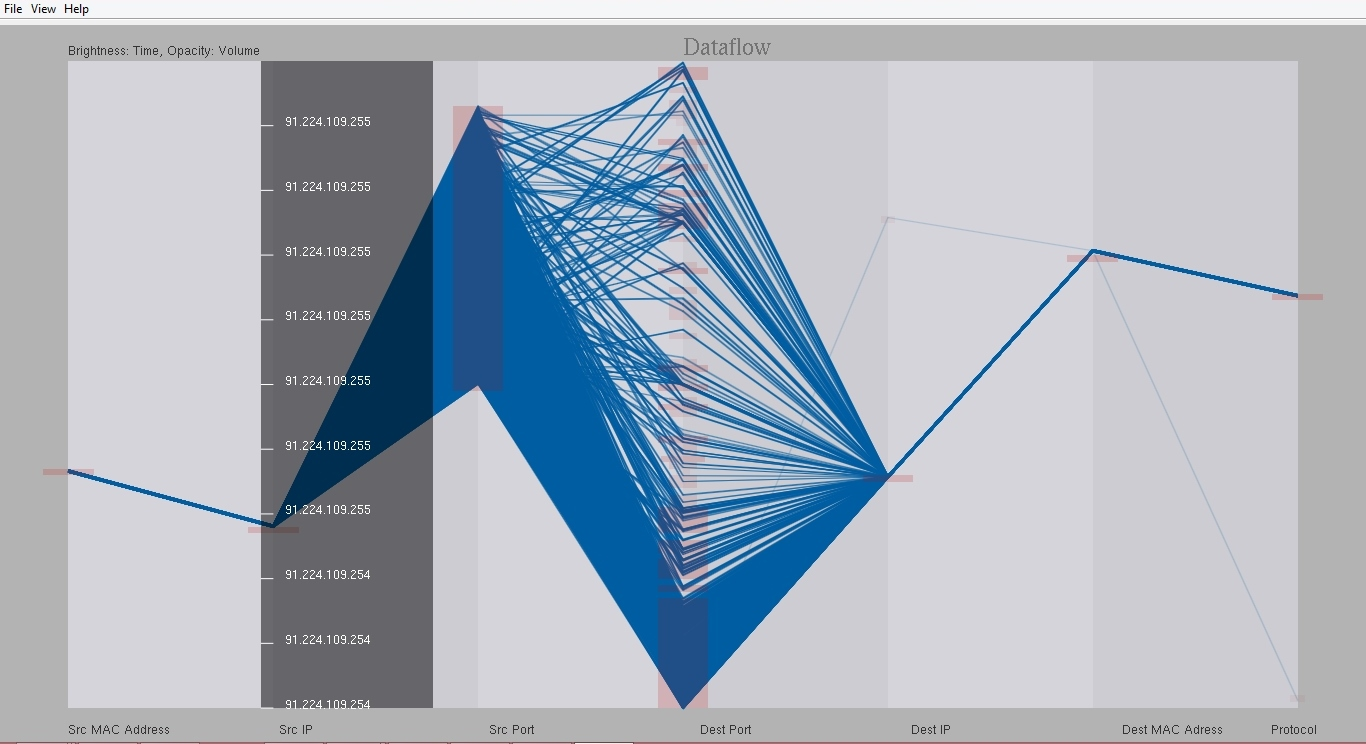
\includegraphics[width=\linewidth]{materials/portscan_explore.jpg}
Applying a range filter isolates the port scan which he can explore further in all the visualizations.

\subsection{Example 2: SSH Attack}

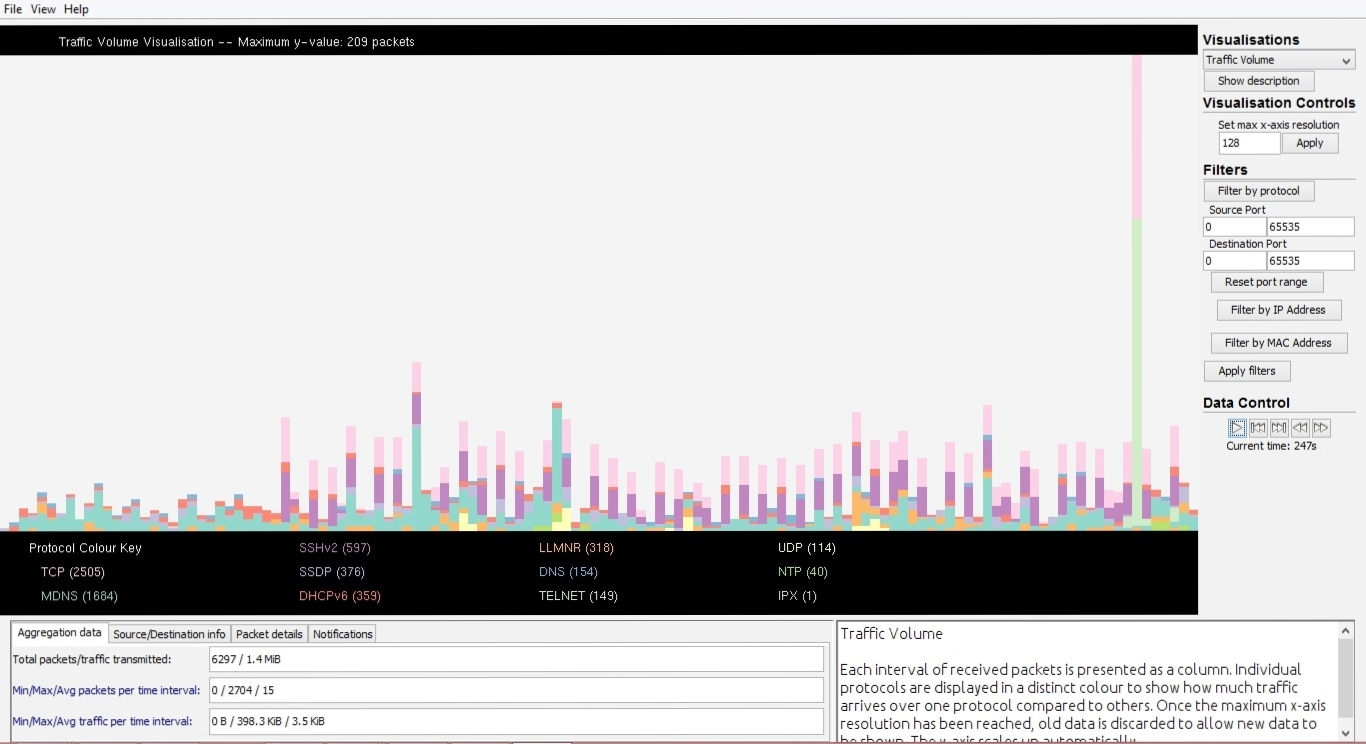
\includegraphics[width=\linewidth]{materials/ssh_suspicious.jpg}
The analyst observes some irregular activity in the traffic volume visualization.

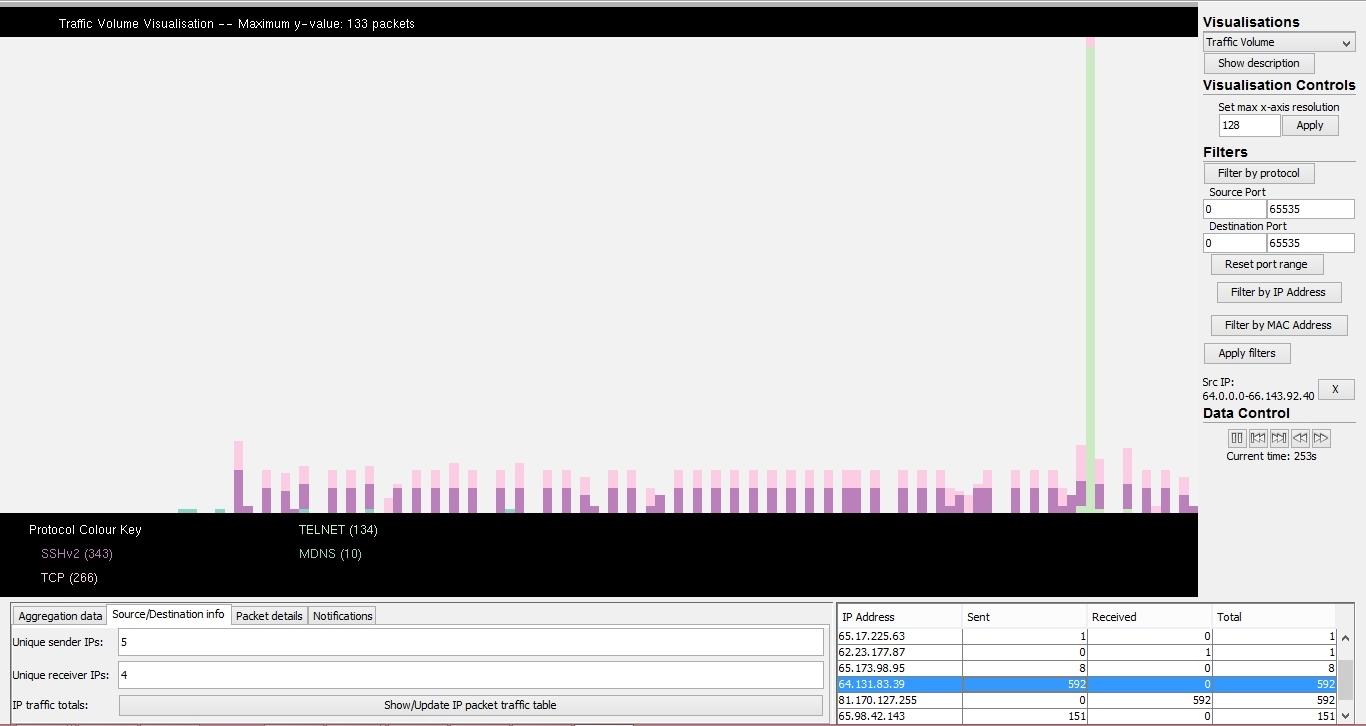
\includegraphics[width=\linewidth]{materials/ssh_explore.jpg}
After exploring with a couple of filters he finds out that a single IP is responsible for all the irregularities. A quick look at the analysis panel provides information about the attacker and the victim. By isolating the packets from the suspicious IP he can determine the type of attack.

\subsection{Summary}
An analyst can train for detecting attacks by using packet captures. After learning the shape of different attacks in each visualization it will become easy for them to detect an ongoing attack. By using different filter combinations they can isolate the attack and learn more about it.

